\chapter{Tự động hóa không chỉ là một công cụ, đó là một cách tư duy}

\begin{infobox}{Quote}
\begin{center}
 "Tự động hóa không chỉ là một công cụ, đó là một cách tư duy."
\end{center}

\end{infobox}

\vspace{1cm}

% \begin{center}
% \textcolor{red}{
% \begin{quote}
%     \itshape
%     "Tự động hóa không chỉ là một công cụ, đó là một cách tư duy."
% \end{quote}
% }
% \end{center}

Chúc mừng bạn! Nếu bạn đang đọc những dòng này, có thể bạn đã hoàn thành phần lớn cuốn sách – một hành trình khám phá đầy thú vị cùng \texttt{n8n}.

Từ việc hiểu giao diện kéo-thả đơn giản, đến xây dựng những workflow phức tạp, tích hợp REST API, xử lý dữ liệu, sử dụng webhook, cron job, rồi triển khai trên server thật – bạn đã có trong tay những kỹ năng nền tảng cực kỳ vững chắc.

\texttt{n8n} không còn là một công cụ xa lạ. Với bạn, nó đã trở thành \textbf{người cộng sự thầm lặng}, âm thầm xử lý hàng chục công việc mỗi ngày – chính xác, nhanh chóng, và không bao giờ than phiền.

\vspace{1em}

Thế giới tự động hóa không có điểm kết thúc. Đó là một dòng chảy liên tục – nơi bạn luôn có thể cải tiến thêm, tối ưu hơn, và nghĩ xa hơn những gì bạn đã làm được.

Hãy tưởng tượng:

\begin{itemize}
    \item Một hệ thống tự động xử lý đơn hàng từ website, gửi email xác nhận, tạo hóa đơn, cập nhật kho, và gửi dữ liệu cho kế toán – tất cả chỉ với \textbf{một lần khách hàng nhấn nút ``Mua hàng''}.
    \item Một bot ChatGPT tích hợp \texttt{n8n}, tự động đọc email, hiểu nội dung, phân loại và phản hồi khách hàng.
    \item Một doanh nghiệp không còn bộ phận nhập liệu thủ công, vì \texttt{n8n} đã làm thay họ toàn bộ.
\end{itemize}

Chúng không còn là tương lai – chúng đang diễn ra \textbf{ngay lúc này}.

\vspace{1em}

\texttt{n8n} rất mạnh khi đứng một mình – nhưng còn mạnh hơn nữa khi bạn biết \textbf{kết hợp nó với các công cụ khác} như:

\begin{itemize}
    \item \textbf{Airtable / Notion / Google Sheet}: Quản lý cơ sở dữ liệu dạng bảng cực kỳ trực quan.
    \item \textbf{ChatGPT / OpenAI}: Xử lý ngôn ngữ, phân tích văn bản, tổng hợp báo cáo.
    \item \textbf{Make.com / Zapier}: Nếu một số tích hợp \texttt{n8n} chưa có, bạn vẫn có thể mix giữa các nền tảng.
    \item \textbf{Slack / Telegram / Discord}: Giao tiếp, gửi thông báo, điều khiển từ xa qua chatbot.
    \item \textbf{Docker / GitHub / CI/CD}: Quản lý và triển khai tự động hệ thống của bạn.
\end{itemize}

Việc kết nối các công cụ này tạo nên một \textbf{hệ sinh thái no-code / low-code mạnh mẽ}, có thể vận hành toàn bộ một doanh nghiệp vừa và nhỏ.

\vspace{1em}

Tự động hóa không chỉ là tiết kiệm thời gian. Nó là một \textbf{triết lý làm việc}:

\begin{itemize}
    \item Loại bỏ việc lặp đi lặp lại.
    \item Giải phóng trí óc khỏi những công việc nhỏ.
    \item Tập trung vào những gì thực sự có giá trị: sáng tạo, kết nối con người, xây dựng chiến lược.
\end{itemize}

Một người làm việc hiệu quả không phải vì họ giỏi làm nhiều thứ – mà vì họ giỏi \textit{không cần làm những thứ không cần thiết nữa}.

\vspace{1em}

Từ đây, bạn có thể chọn những hướng đi xa hơn với \texttt{n8n}:

\begin{itemize}
    \item \textbf{Tự viết node riêng} cho các phần mềm nội bộ.
    \item \textbf{Đóng góp mã nguồn mở}, sửa lỗi, phát triển tính năng.
    \item \textbf{Xây dựng sản phẩm} từ workflow và bán cho người khác.
    \item \textbf{Triển khai quy mô lớn} với Docker, ECS, Kubernetes.
    \item \textbf{Trở thành chuyên gia}, tư vấn cho doanh nghiệp, dạy lại người khác.
\end{itemize}

\vspace{1em}


\newpage
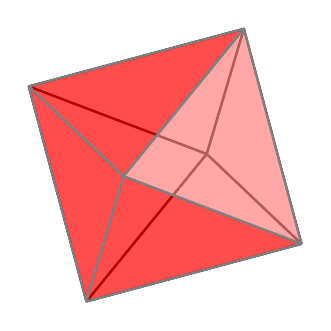
\begin{tikzpicture}[thick,scale=2,line join=bevel,z=-5.5, rotate = -30]
\coordinate (A1) at (0,0,-1);
\coordinate (A2) at (-1,0,0);
\coordinate (A3) at (0,0,1);
\coordinate (A4) at (1,0,0);
\coordinate (B1) at (0,1,0);
\coordinate (C1) at (0,-1,0);

\draw (A1) -- (A2) -- (B1) -- cycle;
\draw (A4) -- (A1) -- (B1) -- cycle;
\draw (A1) -- (A2) -- (C1) -- cycle;
\draw (A4) -- (A1) -- (C1) -- cycle;
\draw [thick,black!50,fill opacity=0.7,fill=red] (A2) -- (A3) -- (B1) -- cycle;
\draw [black!50,fill opacity=0.7,fill=red!50] (A3) -- (A4) -- (B1) -- cycle;
\draw [black!50,fill opacity=0.7,fill=red] (A2) -- (A3) -- (C1) -- cycle;
\draw [black!50,fill opacity=0.7,fill=red] (A3) -- (A4) -- (C1) -- cycle;
\end{tikzpicture}

\section*{Feedback}

Cảm ơn bạn đã dành thời gian đọc cuốn sách này! Nếu bạn có bất kỳ góp ý, câu hỏi, hay đề xuất nội dung nào giúp cải thiện phiên bản tiếp theo, chúng tôi rất mong nhận được phản hồi từ bạn.
\begin{center}
    
\begin{mynote} 
Quét mã QR bên dưới để gửi phản hồi trực tiếp. Hoặc trực tiếp qua link sau: \href{https://docs.google.com/forms/d/e/1FAIpQLSdcaJhbDg3Xu_x7aAFVxZJlK0dm-nBmFMbjgaEURXB1C8engw/viewform?usp=dialog}{link}: 


\includegraphics[width=0.8\linewidth]{Chap1-7/qrcode.pdf}

 \begin{itemize}[label=\small\rhombusdot]
 \item Nội dung có dễ hiểu không?
 \item Bạn muốn thêm chủ đề gì?
 \item Đánh giá giúp mình nhé!
 \end{itemize}
\end{mynote} 

\end{center}


